% (find-LATEX "2020-1-C2-somas-2.tex")
% (defun c () (interactive) (find-LATEXsh "lualatex -record 2020-1-C2-somas-2.tex" :end))
% (defun D () (interactive) (find-pdf-page      "~/LATEX/2020-1-C2-somas-2.pdf"))
% (defun d () (interactive) (find-pdftools-page "~/LATEX/2020-1-C2-somas-2.pdf"))
% (defun e () (interactive) (find-LATEX "2020-1-C2-somas-2.tex"))
% (defun u () (interactive) (find-latex-upload-links "2020-1-C2-somas-2"))
% (defun v () (interactive) (find-2a '(e) '(d)) (g))
% (find-pdf-page   "~/LATEX/2020-1-C2-somas-2.pdf")
% (find-sh0 "cp -v  ~/LATEX/2020-1-C2-somas-2.pdf /tmp/")
% (find-sh0 "cp -v  ~/LATEX/2020-1-C2-somas-2.pdf /tmp/pen/")
%   file:///home/edrx/LATEX/2020-1-C2-somas-2.pdf
%               file:///tmp/2020-1-C2-somas-2.pdf
%           file:///tmp/pen/2020-1-C2-somas-2.pdf
% http://angg.twu.net/LATEX/2020-1-C2-somas-2.pdf
% (find-LATEX "2019.mk")

% «.defs»		(to "defs")
% «.title»		(to "title")
% «.exercicio-1»	(to "exercicio-1")
% «.exercicio-2»	(to "exercicio-2")
% «.exercicio-7-sup»	(to "exercicio-7-sup")

\documentclass[oneside,12pt]{article}
\usepackage[colorlinks,citecolor=DarkRed,urlcolor=DarkRed]{hyperref} % (find-es "tex" "hyperref")
\usepackage{amsmath}
\usepackage{amsfonts}
\usepackage{amssymb}
\usepackage{pict2e}
\usepackage[x11names,svgnames]{xcolor} % (find-es "tex" "xcolor")
%\usepackage{colorweb}                 % (find-es "tex" "colorweb")
%\usepackage{tikz}
%
% (find-dn6 "preamble6.lua" "preamble0")
%\usepackage{proof}   % For derivation trees ("%:" lines)
%\input diagxy        % For 2D diagrams ("%D" lines)
%\xyoption{curve}     % For the ".curve=" feature in 2D diagrams
%
\usepackage{edrx15}               % (find-LATEX "edrx15.sty")
\input edrxaccents.tex            % (find-LATEX "edrxaccents.tex")
\input edrxchars.tex              % (find-LATEX "edrxchars.tex")
\input edrxheadfoot.tex           % (find-LATEX "edrxheadfoot.tex")
\input edrxgac2.tex               % (find-LATEX "edrxgac2.tex")
%
%\usepackage[backend=biber,
%   style=alphabetic]{biblatex}            % (find-es "tex" "biber")
%\addbibresource{catsem-slides.bib}        % (find-LATEX "catsem-slides.bib")
%
% (find-es "tex" "geometry")
\usepackage[a6paper, landscape,
            top=1.5cm, bottom=.25cm, left=1cm, right=1cm, includefoot
           ]{geometry}
%
\begin{document}

\catcode`\^^J=10
\directlua{dofile "dednat6load.lua"}  % (find-LATEX "dednat6load.lua")

% %L dofile "edrxtikz.lua"  -- (find-LATEX "edrxtikz.lua")
% %L dofile "edrxpict.lua"  -- (find-LATEX "edrxpict.lua")
% \pu

% «defs»  (to ".defs")
% (find-LATEX "edrx15.sty" "colors-2019")
\long\def\ColorRed   #1{{\color{Red1}#1}}
\long\def\ColorViolet#1{{\color{MagentaVioletLight}#1}}
\long\def\ColorViolet#1{{\color{Violet!50!black}#1}}
\long\def\ColorGreen #1{{\color{SpringDarkHard}#1}}
\long\def\ColorGreen #1{{\color{SpringGreenDark}#1}}
\long\def\ColorGreen #1{{\color{SpringGreen4}#1}}
\long\def\ColorGray  #1{{\color{GrayLight}#1}}
\long\def\ColorGray  #1{{\color{black!30!white}#1}}
\long\def\ColorBrown #1{{\color{Brown}#1}}
\long\def\ColorBrown #1{{\color{brown}#1}}

\long\def\ColorShort #1{{\color{SpringGreen4}#1}}
\long\def\ColorLong  #1{{\color{Red1}#1}}

\def\frown{\ensuremath{{=}{(}}}
\def\True {\mathbf{V}}
\def\False{\mathbf{F}}
\def\sup  {\mathsf{sup}}
\def\inf  {\mathsf{inf}}

\def\drafturl{http://angg.twu.net/LATEX/2020-1-C2.pdf}
\def\drafturl{http://angg.twu.net/2020.1-C2.html}
\def\draftfooter{\tiny \href{\drafturl}{\jobname{}} \ColorBrown{\shorttoday{} \hours}}

% (find-angg ".emacs" "c2q192")


%  _____ _ _   _                               
% |_   _(_) |_| | ___   _ __   __ _  __ _  ___ 
%   | | | | __| |/ _ \ | '_ \ / _` |/ _` |/ _ \
%   | | | | |_| |  __/ | |_) | (_| | (_| |  __/
%   |_| |_|\__|_|\___| | .__/ \__,_|\__, |\___|
%                      |_|          |___/      
%
% «title»  (to ".title")

\thispagestyle{empty}

\begin{center}

\vspace*{1.2cm}

{\bf \Large Cálculo 2 - 2020.1}

\bsk

Aulas 3 e 4: Integrais como somas de retângulos (2)

\bsk

Eduardo Ochs - RCN/PURO/UFF

\url{http://angg.twu.net/2020.1-C2.html}

\end{center}

\newpage

{\bf Aproximações por cima e por baixo}

Uma das figuras na p.2 das notas da Cristiane Hernández é esta:

% (find-books "__analysis/__analysis.el" "hernandez")
% (find-c2crishernandezpage (+ 10  2) "")
% (find-latexgimp-links "2020-1-C2/area-hernandez-1")

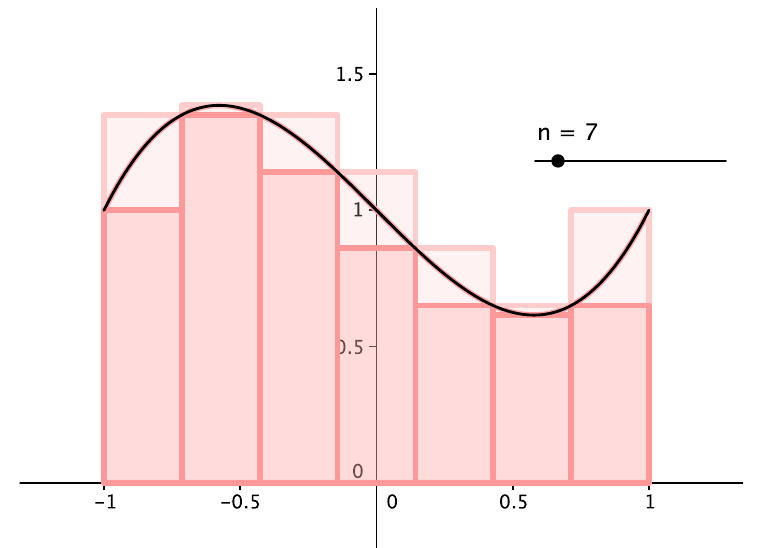
\includegraphics[width=6cm]{2020-1-C2/area-hernandez-1.png}

Ela mostra uma tentativa de calcular uma integral fazendo uma {\sl
  aproximação por retângulos por baixo} e uma {\sl aproximação por
  retângulos por cima} para $y=f(x)$ no intervalo entre $x=-1$ e
$x=1$. A curva $y=f(x)$ fica entre estas duas aproximações.

\newpage

% «exercicio-1»  (to ".exercicio-1")
% (c2m201somas2p 3 "exercicio-1")
% (c2m201somas2    "exercicio-1")

{\bf Exercício 1.}

Sejam $g(x)=5-x$ e $P=\{1,2,4\}$.

Considere a expressão abaixo:
%
$$\sum_{i=1}^N g(b_i)(b_i-a_i)
  ≤ \Intx{1}{4}{g(x)}
  ≤ \sum_{i=1}^N g(a_i)(b_i-a_i)
  \qquad
  (*)
$$

a) Represente graficamente o primeiro somatório e calcule-o.

b) Represente graficamente o segundo somatório e calcule-o.

c) Represente graficamente a integral $\Intx{1}{4}{g(x)}$ como a área
sob a curva $y=g(x)$ entre $x=1$ e $x=4$ e calcule-a -- lembre que
vimos no final da aula passada como calcular áreas de trapézios.

d) Verifique que os dois `$≤$'s em $(*)$ são verdade.

e) Represente os dois somatórios e a integral num gráfico só.


\newpage

{\bf Exercício 1 (continuação).}

\ssk

f) O primeiro somatório está todo abaixo da curva $y=g(x)$? A curva
$y=g(x)$ está toda abaixo do segundo somatório? Se ``sim'' e ``sim''
represente os dois somatórios e a integral num gráfico só fazendo uma
figura parecida com a do slide 2, inclusive usando cores diferentes
para a área sob a aproximação por baixo (o somatório da esquerda) e a
aproximação por cima (o somatório da direita).


\newpage

Nos próximos exercícios nós vamos encontrar modos de fazer
aproximações por retângulos ``por cima'' e ``por baixo''. As nossas
primeiras tentativas vão ser meio bugadas e vai ser preciso
consertá-las.

Lembre que na aula passada nós vimos como visualizar vários somatórios
diferentes, e os que apareceram no exercício 1 correspondem à ``soma à
direita'' e a ``soma à esquerda'' desta página da Wikipedia:

\ssk

\url{https://pt.wikipedia.org/wiki/Soma_de_Riemann}

\newpage

% (c2m192p 3 "retangulos")
% (c2m192    "retangulos")

{\bf Algumas abreviações}

\def\sumiN#1{\sum_{i=1}^N #1 (b_i-a_i)}
\def\mname#1{\text{[#1]}}

$$\begin{array}{ccl}
  \mname{L}    &=& \sumiN {f(a_i)} \\
  \mname{R}    &=& \sumiN {f(b_i)} \\
  \mname{Trap} &=& \sumiN {\frac{f(a_i) + f(b_i)}{2}} \\
  \mname{M}    &=& \sumiN {f(\frac{a_i+b_i}{2})} \\
  \mname{min}  &=& \sumiN {\min(f(a_i), f(b_i))} \\
  \mname{max}  &=& \sumiN {\max(f(a_i), f(b_i))} \\
  % [5pt]
  % \mname{inf}  &=& \sumiN {\inf (\setofst{f(x)}{x∈[a_i,b_i]}) } \\
  % \mname{sup}  &=& \sumiN {\sup (\setofst{f(x)}{x∈[a_i,b_i]}) } \\
  % [5pt]
  % \overline \int_P f(x) \, dx &=& \sumiN {\sup (\setofst{f(x)}{x∈[a_i,b_i]}) } \\
  % \underline\int_P f(x) \, dx &=& \sumiN {\inf (\setofst{f(x)}{x∈[a_i,b_i]}) } \\
\end{array}
$$

Obs: todos os ``métodos'' acima, $\mname{L}$, $\mname{R}$,
$\mname{Trap}$, $\mname{M}$, $\mname{min}$, e $\mname{max}$, aparecem
na página da Wikipedia, mas com outros nomes e usando partições em que
todos os subintervalos têm o mesmo comprimento!

\newpage

% «exercicio-2»  (to ".exercicio-2")
% (c2m201somas2p 7 "exercicio-2")
% (c2m201somas2    "exercicio-2")

{\bf Exercício 2.} Seja $f$ a nossa função preferida (a da aula
passada!) e $P$ a partição $P=\{1,1.5,2,3,4\}$.

a) Represente em um gráfico só a função $f$ e $\mname{M}$.

b) Represente em um gráfico só a função $f$ e $\mname{min}$.

c) Represente em um gráfico só a função $f$ e $\mname{max}$.

\bsk

{\bf Exercício 3.} Faça um gráfico como o do item (f) do exercício 1
para
%
$$\mname{min} ≤ \Intx{1}{4}{f(x)} ≤ \mname{max}.$$

\bsk

{\bf Exercício 4.} Faça um gráfico como o do exercício anterior, mas
agora usando $P=\{1,1.5,3,4\}$. \ColorRed{Desta vez um trecho do
  gráfico de $y=f(x)$ vai ficar acima do \mname{max}!!!}



\newpage

{\bf A imagem de um conjunto por uma função}

Sejam:
%
$$\begin{array}{rcl}
  A &=& \{1,1.5,2,3\} \\
  B &=& \setofst{(x,f(x))}{x∈A} \\ 
    &=& \{ (1,f(1)), (1.5,f(1.5)), (2,f(2)), (3,f(3)) \} \\ 
  C &=& \setofst{f(x)}{x∈A} \\ 
    &=& \{ f(1), f(1.5), f(2), f(3) \} \\ 
  \end{array}
$$

Dá pra desenhar todos esses conjuntos num gráfico só bem rápido.

Instruções: desenhe o gráfico de $y=f(x)$; represente $A$ no eixo $x$;
desenhe $B$ em $\R^2$ ``levantando os pontos de $A$ para a curva de
$y=f(x)$''; represente $C$ \ColorRed{no eixo $y$} ``projetando os
pontos de $B$ no eixo $y$''.

\msk

{\bf Exercício 5.} Faça esse gráfico.

{\bf Exercício 6.} Faça a mesma coisa, mas com $A=[1,3.5]$, que é um
conjunto \ColorRed{infinito}... agora o conjunto $C$ vai ser um
intervalo. Qual?

\newpage

{\bf Um abuso de linguagem}

\ssk

A nossa função $f$ preferida é
%
$$\begin{array}{rrcl}
  f: & \R &→& \R \\
     &  x &↦& 4-(x-2)^2 \\
  \end{array}
$$

O domínio dela é $\R$, e isso quer dizer que se ela receber qualquer
argumento que não é um elemento de $\R$ ela deve dar erro...

Existe um truque tradicional que nos permite escrever a imagem de um
conjunto por uma função de um jeito mais curto. Se $A⊆\R$ é um
conjunto,
%
$$ f(A) = \setofst{f(a)}{a∈A} $$

É como se estivéssemos definindo uma função $f$ nova a partir da $f$
original, e as duas tem o mesmo nome mas domínios disjuntos -- a
original só lida com argumentos que são números reais, e a nova só
lida com argumentos que são conjuntos de números.


\newpage

% «exercicio-7-sup»  (to ".exercicio-7-sup")
% (c2m201somas2p 10 "exercicio-7-sup")
% (c2m201somas2     "exercicio-7-sup")

{\bf Sup}

\ssk

A função $\sup$ é uma espécie de generalização do $\mathsf{max}$.

Vamos começar com um exemplo. No exercício 6 você ``calculou'' -- por
desenhos e olhômetro -- $f([1,3.5])$, e você obteve um intervalo no
eixo $y$. Sejam $A=[1,3.5]$ e $C=f(A)$. Seja
%
$$D = \setofst{y∈\R∪\{-∞,+∞\}}{∀c∈C.\, c≤y}.$$

{\bf Exercício 7.} É verdade que $4∈D$?

{\bf Exercício 8.} É verdade que $5∈D$?

{\bf Exercício 9.} É verdade que $2∈D$?

{\bf Exercício 10.} É verdade que $+∞∈D$?

{\bf Exercício 11.} É verdade que $-∞∈D$?

{\bf Exercício 12.} Represente graficamente o conjunto $D$.

{\bf Exercício 13.} Qual é o menor elemento de $D$?

\newpage

{\bf Sup (2)}

\ssk

A definição \ColorRed{formal} do $\sup$ é \ColorRed{bem} complicada...

Dê uma olhada nesta página da Wikipedia, como curiosidade:

\ssk

\url{https://pt.wikipedia.org/wiki/Supremo_e_\%C3\%ADnfimo}

\ssk

Quando $C⊆\R$ temos um procedimento pra calcular $\sup(C)$ que é
equivalente à definição ``oficial'' complicadíssima que aparece na
Wikipedia. Ele funciona assim: defina
%
$$D = \setofst{y∈\R∪\{-∞,+∞\}}{∀c∈C.\, c≤y}.$$

Este conjunto $D$ vai ter duas propriedades importantes:

1) se $d∈D$ então $[d,+∞)⊆D$, e

2) $D$ tem um menor elemento.

\msk

O resultado de $\sup(C)$ vai ser o menor elemento de $D$.

\newpage

{\bf Sup e Inf}

\ssk

A definição \ColorRed{informal} abaixo também funciona:

Se $C⊆\R$ então $\sup(C)$ é o menor elemento de $\R∪\{-∞,∞\}$ que está
``\ColorRed{acima}'' de todos os elementos de $C$.

\msk

e, similarmente...

\msk

Se $C⊆\R$ então $\inf(C)$ é o maior elemento de $\R∪\{-∞,∞\}$ que está
``\ColorRed{abaixo}'' de todos os elementos de $C$.


\bsk


{\bf Exercício 14.} Calcule:

\def\foo#1{$\sup(#1)$ e $\inf(#1)$}

a) \foo{\{2,3,4\}}

b) \foo{[2,4]}

c) \foo{(2,4)}

d) \foo{\R}

e) \foo{∅}

\newpage


{\bf Algumas abreviações (2)}

\def\sumiN#1{\sum_{i=1}^N #1 (b_i-a_i)}
\def\mname#1{\text{[#1]}}

$$\begin{array}{ccl}
  \mname{L}    &=& \sumiN {f(a_i)} \\
  \mname{R}    &=& \sumiN {f(b_i)} \\
  \mname{Trap} &=& \sumiN {\frac{f(a_i) + f(b_i)}{2}} \\
  \mname{M}    &=& \sumiN {f(\frac{a_i+b_i}{2})} \\
  \mname{min}  &=& \sumiN {\min(f(a_i), f(b_i))} \\
  \mname{max}  &=& \sumiN {\max(f(a_i), f(b_i))} \\
  [5pt]
  \mname{inf}  &=& \sumiN {\inf (f([a_i,b_i]) } \\
  \mname{sup}  &=& \sumiN {\sup (f([a_i,b_i]) } \\
  % [5pt]
  % \overline \int_P f(x) \, dx &=& \sumiN {\sup (\setofst{f(x)}{x∈[a_i,b_i]}) } \\
  % \underline\int_P f(x) \, dx &=& \sumiN {\inf (\setofst{f(x)}{x∈[a_i,b_i]}) } \\
\end{array}
$$

Os métodos $\mname{inf}$ e  $\mname{sup}$ são novos...

Eles correspondem ao que a página da Wikipedia chama de ``Soma de
Riemann Inferior'' e ``Soma de Riemann Superior''.



\newpage

{\bf Uma versão ``consertada'' do exercício 4}

\ssk

{\bf Exercício 15.} Seja $P=\{1,1.5,3,4\}$. Faça um gráfico como o do
item (f) do exercício 1 para
%
$$\mname{inf} ≤ \Intx{1}{4}{f(x)} ≤ \mname{sup}.$$

e verifique que agora a curva $y=f(x)$ está entre $\mname{inf}$ e
$\mname{sup}$.













%\printbibliography

\end{document}

%  __  __       _        
% |  \/  | __ _| | _____ 
% | |\/| |/ _` | |/ / _ \
% | |  | | (_| |   <  __/
% |_|  |_|\__,_|_|\_\___|
%                        
% <make>

 (eepitch-shell)
 (eepitch-kill)
 (eepitch-shell)
# (find-LATEXfile "2019planar-has-1.mk")
make -f 2019.mk STEM=2020-1-C2-somas-2 veryclean
make -f 2019.mk STEM=2020-1-C2-somas-2 pdf

% Local Variables:
% coding: utf-8-unix
% ee-tla: "c2m201somas2"
% End:
